\section{方法比较}
\label{sec:feas-compare}

前面四种方法该怎样选？本节先按集合结构筛选，再谈成本。比较的前提是同一个问题确实满足所比较方法的条件，并且用相同的可行精度和相同的最优性度量。

\paragraph{先看集合}
选择的第一步是问集合支持什么运算。闭凸集合上可以选投影、线性最小化或Bregman子问题；光滑非线性等式约束只有GRG的局部消元和解方程这条路，前三种方法的保证不适用。反过来，单纯形这样的简单集合也用不着GRG。把适用集合不同的方法排成统一的优劣次序没有意义。

\paragraph{同一问题上的比较}
三种闭凸方法都能解预算例。图~\ref{fig:feas-compare}(a)显示投影梯度最快，因为投影的代价在单纯形上很低，解又落在一条边上，活动集识别后就是一维问题。

图~\ref{fig:feas-compare}(b)换成高维单纯形上的最小二乘问题，看解的稀疏性。条件梯度的非零元个数从一开始缓慢增长，始终很少；投影梯度从稠密起点迅速截断；镜像下降一直保持全部为正。条件梯度的稀疏只是说输出的表示短，并不说明它更准确。

\begin{BookInlineFigure}
  \centering
  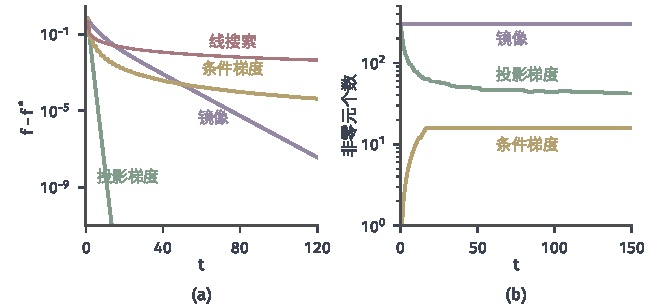
\includegraphics[width=112mm]{figures/05-optimization/06-constrained-optimization/matplotlib/feas-compare/figure.pdf}
  \caption{同一单纯形问题上的比较。(a)预算例的迄今最小目标差：绿线投影梯度，紫线镜像下降，黄线条件梯度（预定序列），红线条件梯度（线搜索）。(b)$n=300$的单纯形最小二乘，随机矩阵$\bm{A}\in\mathbb{R}^{60\times300}$（种子固定），绿线投影梯度和紫线镜像下降从均匀分布出发，黄线条件梯度从一个顶点出发，纵轴是非零元个数。}
  \label{fig:feas-compare}
\end{BookInlineFigure}

表~\ref{tab:feas-compare}归纳了单纯形上每轮的成本和结构。总成本是每轮成本乘以达到相同精度所需的轮数，只看其中一个因子会得出错误的结论。

\begin{BookInlineTable}
  \centering
  \caption{$n$维单纯形上三种方法每轮的额外运算（梯度计算另计）。}
  \label{tab:feas-compare}
  \begin{tabular}{llll}
   \toprule
   方法 & 额外运算 & 输出结构 & 活动约束\\
   \midrule
   投影梯度 & 排序，$O(n\log n)$ & 可稀疏 & 有限步后常被识别\\
   条件梯度 & 找最小分量，$O(n)$ & 顶点的短组合 & 基本流程难以识别\\
   镜像下降 & 乘法与归一化，$O(n)$ & 全部为正 & 不精确识别\\
   \bottomrule
  \end{tabular}
\end{BookInlineTable}

\subsection{内层精度}
\label{sec:feas-compare-inner}

每种方法的子问题都可能只能近似求解。这些内层误差分别影响哪里，又该解到多准？

\paragraph{误差进入的位置}
表~\ref{tab:feas-inner}按方法列出内层误差的去向。投影和GRG的恢复直接影响可行性，线性最小化的误差只影响下降和证书，因为不精确的顶点仍在集合内。

\begin{BookInlineTable}
  \centering
  \caption{内层误差的影响。}
  \label{tab:feas-inner}
  \begin{tabular}{llll}
   \toprule
   内层计算 & 可行性 & 下降 & 停止检验\\
   \midrule
   投影 & 可能略不可行 & 式~\eqref{eq:feas-inexact-recursion} & 残差误差$\varepsilon/\alpha$\\
   线性最小化 & 不受影响 & 式~\eqref{eq:feas-inexact-lmo} & 间隙加$\varepsilon$\\
   镜像子问题 & 视解法而定 & 三点关系多余项 & 同步记录误差\\
   GRG恢复 & 残差至多$\varepsilon_c$ & $F$的值有误差 & 须检查$\bm{c}$\\
   \bottomrule
  \end{tabular}
\end{BookInlineTable}

熵势在单纯形上的子问题有闭式解，归一化的舍入误差可以忽略。一般的集合上，镜像子问题也要迭代求解，并且三点关系~\eqref{eq:feas-three-point}多出误差项，处理方式和近似投影类似。

\paragraph{按外层精度安排内层}
外层离解还远时，把内层解到很高的精度是浪费；外层接近收敛时，内层误差又会成为瓶颈。前面的递推说明了这一点：式~\eqref{eq:feas-inexact-lmo}让线性最小化的容差随$\alpha^{(t)}$减小，式~\eqref{eq:feas-inexact-recursion}说明投影容差决定了误差的平台。常用做法是把内层容差设成外层当前残差的一个比例。

GRG的恢复容差则有一个硬性的下限要求：它决定了输出点的可行程度，至少要达到最终要求的约束精度。

\paragraph{成本要算全}
GRG每轮的成本不只是外层更新，要把下面各项都算进去：
\begin{itemize}
 \item 线搜索中重复的恢复，每次试探步长都要解一次非线性方程；
 \item 每次恢复中的Newton迭代，各需一次约束计算和一次线性方程求解；
 \item Jacobian矩阵的更新与$\bm{B}$的分解，稠密时分解约需$p^3$量级的运算；
 \item 换基之后的重新分解或分解修正。
\end{itemize}

上面圆周例的第三轮就要试探五个步长，其中四个失败或被拒绝，这些计算都要计入总成本。投影梯度的回溯同样要计入重复投影的次数。比较方法时，统计的是这些基本运算的总次数，而不是外层轮数。

\subsection{结果检验}
\label{sec:feas-compare-check}

算法停下来之后，应该报告什么数字来证明结果可用？

\paragraph{凸问题}
凸问题可以报告目标差的上界。条件梯度的间隙$\Gamma$直接就是这样的上界。单纯形上计算$\Gamma$只要$O(n)$，投影梯度或镜像下降也可以顺便算一个间隙作为证书。

没有线性最小化可用时，投影残差也能给出上界。在定理~\ref{thm:feas-pgd-convex}的证明中取$\mu=0$，$\alpha=1/L$，$\bm{y}=\bm{x}^\star$，由内积的上界和残差的定义，得到
\begin{equation}
 f(\bm{x}^{+})-f^\star\leq\lVert\bm{G}_\alpha(\bm{x})\rVert_2\lVert\bm{x}^{+}-\bm{x}^\star\rVert_2+\frac{1}{2L}\lVert\bm{G}_\alpha(\bm{x})\rVert_2^2.
 \label{eq:feas-residual-gap}
\end{equation}
这需要知道到解的距离的上界，比如集合的直径，否则残差小不能换算成目标差小。

\paragraph{非凸光滑问题}
目标非凸时报告驻定度量，$\lVert\bm{G}_\alpha\rVert_2$或$\Gamma$都可以，同时要说明步长，并明确它只检验一阶条件。

\paragraph{GRG}
GRG的报告必须回到原问题的形式：$\lVert\bm{c}(\bm{x})\rVert_\infty$、界的违反量、以及完整的KKT残差。只看约化梯度的范数是不够的。在圆周例的不可行点$(y,z)=(2,0)$上，公式~\eqref{eq:feas-reduced-gradient}算出$\nabla F=0$，而约束残差是$3$。约化梯度的含义依赖于“当前点在约束面上”这个前提。

\paragraph{随机方向}
大规模时梯度常常用随机估计代替。第~\ref{chap:stochastic-gradient-methods}章的分析依赖更新对噪声是线性的，这样条件期望可以直接进入更新。投影和指数映射都是非线性的，期望不能穿过去。

取$\bm{C}=[0,1]$，$x=0$，随机梯度等概率取$\pm1$，期望是零。精确梯度的投影更新留在原地，而随机更新的期望是
\[
 \mathbb{E}\bigl[P_{\bm{C}}(x-\alpha\tilde g)\bigr]=\tfrac12\alpha+\tfrac12\cdot0=\tfrac\alpha2\neq0.
\]

指数映射也是如此：
\[
 \mathbb{E}\bigl[\exp(-\alpha\tilde g)\bigr]=\cosh\alpha>1=\exp\bigl(-\alpha\,\mathbb{E}[\tilde g]\bigr).
\]

所以把随机方向接入投影或镜像更新时，要在变分不等式或三点关系那一层使用条件期望，也就是对内积取期望，然后单独控制噪声带来的二次项，不能把噪声当成在映射之外平均掉。
